%**************************************************************************
\section{Introduction} %***************************************************
%**************************************************************************
\begin{frame}{Market Situation}
The real estate market as being one of the main drivers for established economies and their growth, is worth to be analysed for future economists 
\parencite{Leblanc2009}. Otherwise controlled monetary and fiscal policy can't be executed without adverse effects. How important the real estate market is, became obvious after the last financial crisis, when the dependency of housing markets with the financial markets lead the whole worlds economy into a serious recession. Therefore our goal for this project is to analyse the influence of different macroeconomic factors on the biggest housing price index of the USA over the last 20 years.
\end{frame}

\begin{frame}{Goal}
We want to find the macro-economical components of the "S\&P/Case-Shiller Home Price Index", the biggest real estate index for the United States. The S\&P/Case-Shiller Home Price Index is calculated on a "repeated sales" basis, which means the price of the index is calculated by the price changes of concrete houses in a specific period.
Our assumption concerning the important macro-economical factors are, that topics like the following explain the biggest part of the variation of home price indices. We think that the biggest drivers are interest rates, population growth, equity markets, income and inflation.
\end{frame}

%**************************************************************************
\section{Data} %***********************************************************
%**************************************************************************
\begin{frame}{Data}
    The data used is taken from the official FRED website, obtained using their API. It contains various macro-economic factors from 01/2000 until 06/2022, i.e., over 22 years of monthly data. The selection of these variables was based on the understanding of the housing market of the authors. In this section, each variable will be  briefly described.
\end{frame}

\begin{frame}{House Price Index}
    \begin{tabular}{@{}ll@{}}  
        \begin{tabular}{l}
            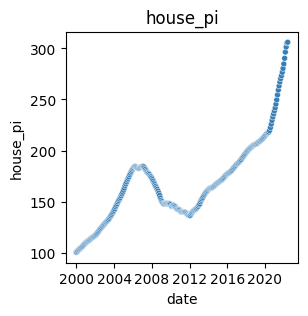
\includegraphics[width = 0.35\linewidth]{images/Graphs/house_pi.png}
        \end{tabular}
        &\begin{tabular}{l}
            \parbox{0.5\linewidth}{%change the parbox width as appropiate
            'house\_pi' has a clearly upwards-sloping trend with a serious uptick in the years leading up to the year 2007/08. This is not surprising as we know today that in the build-up of the subprime crisis real estate prices skyrocketed before the housing price bubble burst. After a short period of price corrections up until ca. the year 2012, the prices have again risen and still are. For the following years we assume that the prices will come back down due to the several interest rate rises which will directly lead to a downward trend for all assets.
            }
        \end{tabular} \\
    \end{tabular}
\end{frame}

\begin{frame}{Consumer Sentiment}
    \begin{tabular}{@{}ll@{}}  
        \begin{tabular}{l}
            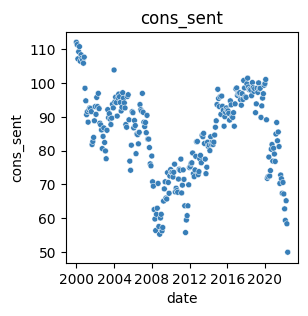
\includegraphics[width = 0.35\linewidth]{images/Graphs/cons_sent.png}
        \end{tabular}
        &\begin{tabular}{l}
            \parbox{0.5\linewidth}{%change the parbox width as appropiate
            'cons\_sent' paints a somewhat cyclical picture, marked by the recessions caused by the big crises in the 21st century thus far. For example the subprime crisis in 2008 caused consumers to have lower faith in the economy and were scared to in invest or buy in general. The same can be observed in the year 2019 when the covid-19 crisis started.
            }
        \end{tabular} \\
    \end{tabular}
\end{frame}

\begin{frame}{Corporate Bond Yield}
    \begin{tabular}{@{}ll@{}}  
        \begin{tabular}{l}
            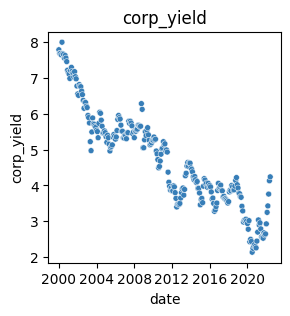
\includegraphics[width = 0.35\linewidth]{images/Graphs/corp_yield.png}
        \end{tabular}
        &\begin{tabular}{l}
            \parbox{0.5\linewidth}{%change the parbox width as appropiate
            'corp\_yield' has a very similar evolution over time as 'mortgage\_int' which is not particularly surprising since for both, the prime rate has a very big impact. Since the central banks in the western world constantly decreased the prime rate over the last two decades, all other interest rates decreased too with an appropriate risk surplus.
            }
        \end{tabular} \\
    \end{tabular}
\end{frame}

\begin{frame}{CPI}
    \begin{tabular}{@{}ll@{}}  
        \begin{tabular}{l}
            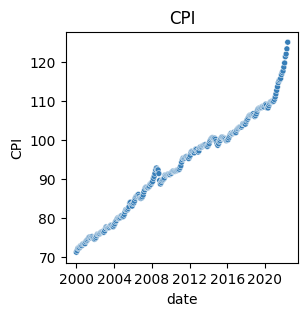
\includegraphics[width = 0.35\linewidth]{images/Graphs/CPI.png}
        \end{tabular}
        &\begin{tabular}{l}
            \parbox{0.5\linewidth}{%change the parbox width as appropiate
            'CPI' has steadily risen since the the beginning of the 21st century. Since and because of the corona pandemic and additionally fuelled by the on-going war in eastern Europe, we have seen major yoy increases in inflation. Central banks around the world have tried to get inflation under control by increasing interest rates which has not shown much effect up to the end of our sample time.
            }
        \end{tabular} \\
    \end{tabular}
\end{frame}

\begin{frame}{Home Supply}
    \begin{tabular}{@{}ll@{}}  
        \begin{tabular}{l}
            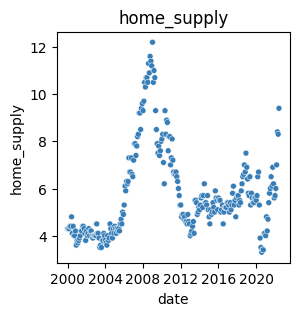
\includegraphics[width = 0.35\linewidth]{images/Graphs/home_supply.png}
        \end{tabular}
        &\begin{tabular}{l}
            \parbox{0.5\linewidth}{%change the parbox width as appropiate
            The 'home\_supply' has a slight upwards-sloping trend with a huge upwards move shortly before the subprime crisis. Notice, that while 'house\_pi' started increasing rapidly after its low point, 'home\_supply' had more of a slow trod before its volatilty started increasing from the year 2020 onwards.
            }
        \end{tabular} \\
    \end{tabular}
\end{frame}

\begin{frame}{Mortgage Interest Rate}
    \begin{tabular}{@{}ll@{}}  
        \begin{tabular}{l}
            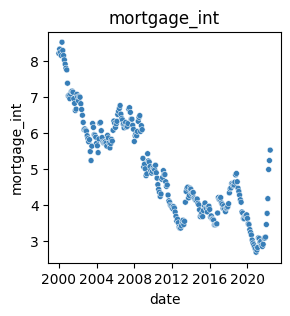
\includegraphics[width = 0.35\linewidth]{images/Graphs/mortgage_int.png}
        \end{tabular}
        &\begin{tabular}{l}
            \parbox{0.5\linewidth}{%change the parbox width as appropiate
            Up until ca. 2020, 'mortagage\_int' exhibits a clear downwards-sloping trend sparked yet again by the recent crises. Since 2020, however, we observe a turnaround which is in close connection to the effort of central banks (especially the FED) to curb inflation. This turnaround marked a historic point for real estate investors due to the fact that the high asset returns for real estate come to an end.
            }
        \end{tabular} \\
    \end{tabular}
\end{frame}

\begin{frame}{NASDAQ}
    \begin{tabular}{@{}ll@{}}  
        \begin{tabular}{l}
            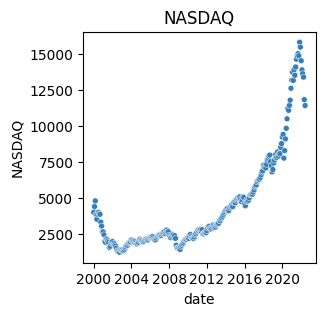
\includegraphics[width = 0.35\linewidth]{images/Graphs/NASDAQ.png}
        \end{tabular}
        &\begin{tabular}{l}
            \parbox{0.5\linewidth}{%change the parbox width as appropiate
            As the second largest stock exchange by market capitalisation, 'NASDAQ' shows very nicely the economic cycle with big crashes following the Dotcom and housing price bubbles at the beginning of the century and following the years 2007/08 respectively. After 2010, the index made great recoveries up until the corona pandemic had great adverse effects on the stock prices yet again. 
            }
        \end{tabular} \\
    \end{tabular}
\end{frame}

\begin{frame}{New Houses}
    \begin{tabular}{@{}ll@{}}  
        \begin{tabular}{l}
            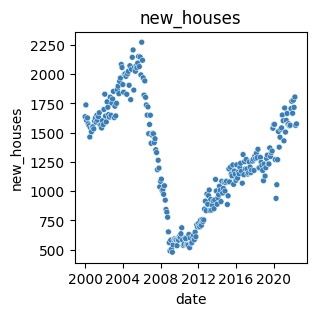
\includegraphics[width = 0.35\linewidth]{images/Graphs/new_houses.png}
        \end{tabular}
        &\begin{tabular}{l}
            \parbox{0.5\linewidth}{%change the parbox width as appropiate
            'new\_houses' had mainly increasing values except for the subprime crisis. After that, the number of new houses for sale have again steadily increased at seemingly the same rate as before the crisis. That is because construction plannings and their execution suffer from the lagging nature of the real estate market. So it can be assumed that this steep curve will turnaround in the near future.
            }
        \end{tabular} \\
    \end{tabular}
\end{frame}

\begin{frame}{Personal Income}
    \begin{tabular}{@{}ll@{}}  
        \begin{tabular}{l}
            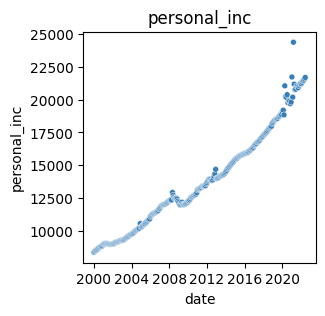
\includegraphics[width = 0.35\linewidth]{images/Graphs/personal_inc.png}
        \end{tabular}
        &\begin{tabular}{l}
            \parbox{0.5\linewidth}{%change the parbox width as appropiate
            'personal\_inc' has experienced a steady upwards-sloping trend since the start date of our data set which obviously follows from the increase in inflation over the past decades. Note, however, that naturally due to the nature of salary negotiations, the line is much smoother compared to the one of 'CPI'.
            }
        \end{tabular} \\
    \end{tabular}
\end{frame}

\begin{frame}{Population}
    \begin{tabular}{@{}ll@{}}  
        \begin{tabular}{l}
            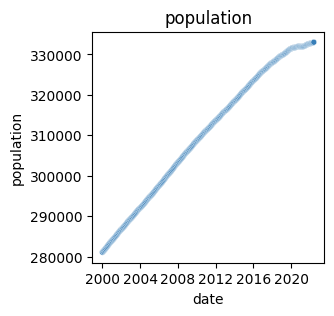
\includegraphics[width = 0.35\linewidth]{images/Graphs/population.png}
        \end{tabular}
        &\begin{tabular}{l}
            \parbox{0.5\linewidth}{%change the parbox width as appropiate
            Unsurprisingly, especially with the latest cornerstone of exceeding eight billion humans only very recently, 'population' has had a steady increase over the entire observed time. The only slight dampening started a short while ago where we can see a decrease in the slope of the trend since approximately 2020.
            }
        \end{tabular} \\
    \end{tabular}
\end{frame}

\begin{frame}{Unemployment Rate}
    \begin{tabular}{@{}ll@{}}  
        \begin{tabular}{l}
            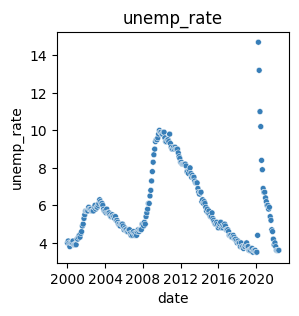
\includegraphics[width = 0.35\linewidth]{images/Graphs/unemp_rate.png}
        \end{tabular}
        &\begin{tabular}{l}
            \parbox{0.5\linewidth}{%change the parbox width as appropiate
            'unemp\_rate' has seen upticks after every major crisis - dotcom bubble in the early 21st century, the financial crisis starting in 2008 and very recently the Corona pandemic.
            }
        \end{tabular} \\
    \end{tabular}
\end{frame}

\begin{frame}{VIX}
    \begin{tabular}{@{}ll@{}}  
        \begin{tabular}{l}
            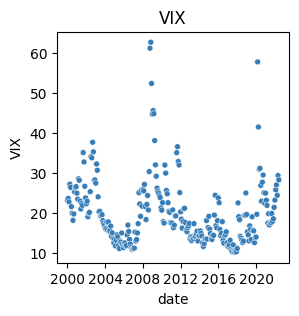
\includegraphics[width = 0.35\linewidth]{images/Graphs/VIX.png}
        \end{tabular}
        &\begin{tabular}{l}
            \parbox{0.5\linewidth}{%change the parbox width as appropiate
            Also the 'VIX' is an indicator of crisis. As is known amongst professionals in the financial industry, volatility increases in turbulent times which is nicely visible for the three big crashes in the last two decades.
            }
        \end{tabular} \\
    \end{tabular}
\end{frame}

\begin{frame}{Working Population}
    \begin{tabular}{@{}ll@{}}  
        \begin{tabular}{l}
            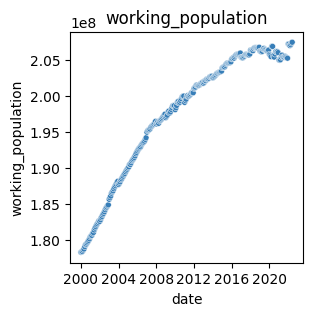
\includegraphics[width = 0.35\linewidth]{images/Graphs/working_population.png}
        \end{tabular}
        &\begin{tabular}{l}
            \parbox{0.5\linewidth}{%change the parbox width as appropiate
            The 'working\_population' obviously follows 'population' very closely with some exceptions after approximately 2020 which surely is (at least to some extent) attributable to the corona crisis where a huge number of people lost their job. In general, one observes a somewhat more rippled line prior to 2020 in comparison to the general population.
            }
        \end{tabular} \\
    \end{tabular}
\end{frame}

%**************************************************************************
\section{Model Fitting} %**************************************************
%**************************************************************************
\begin{frame}{Model 1: All predictors w/o constant}
\scriptsize
\begin{table}[h]
    \centering
    \begin{tabular}{l d{3.3} d{3.3} d{3.3}}
        \hline
        \text{predictor}   &\text{coef}   &\text{std err}    &\text{t} \\
        \hline
        month	 &0.008	 &0.038	 &\textcolor{nicered}{0}.\textcolor{nicered}{203} \\
        year	 &-0.203	 &0.045	 &-4.489 \\
        unemp\_rate	 &-2.517	 &0.55	 &-4.579 \\
        CPI	 &-0.018	 &0.102	 &\textcolor{nicered}{-0}.\textcolor{nicered}{179} \\
        cons\_sent	 &0.009	 &0.057	 &\textcolor{nicered}{0}.\textcolor{nicered}{151} \\
        PI\_const	 &-0.099	 &0.143	 &\textcolor{nicered}{-0}.\textcolor{nicered}{688} \\
        mortgage\_int	 &0.143	 &0.104	 &\textcolor{nicered}{1}.\textcolor{nicered}{372} \\
        personal\_inc	 &1.375	 &0.427	 &3.224 \\
        corp\_yield	 &-0.043	 &0.108	 &\textcolor{nicered}{-0}.\textcolor{nicered}{399} \\
        home\_supply	 &-0.028	 &0.078	 &\textcolor{nicered}{-0}.\textcolor{nicered}{365} \\
        population	 &-0.241	 &0.119	 &-2.019 \\
        new\_houses	 &0.081	 &0.05	 &\textcolor{nicered}{1}.\textcolor{nicered}{612}\\
        working\_population	 &0.286	 &0.149	 &\textcolor{nicered}{1}.\textcolor{nicered}{916} \\
        NASDAQ	 &0.364	 &0.169	 &2.157 \\
        VIX	 &0.151	 &0.136	 &\textcolor{nicered}{1}.\textcolor{nicered}{111} \\
        \hline
    \end{tabular}
    \caption{Model 1.1}
    \label{tab:Model 1.1}
\end{table}
\small
\end{frame}

\begin{frame}{Model 1: All predictors w constant}
\scriptsize
\begin{table}[h]
    \centering
    \begin{tabular}{l d{3.3} d{3.3} d{3.3}}
        \hline
        \text{predictor}   &\text{coef}   &\text{std err}    &\text{t} \\
        \hline
        const	 &0.973	 &0.345	 &2.82 \\
        month	 &0.013	 &0.037	 &\textcolor{nicered}{0}.\textcolor{nicered}{349} \\
        year	 &-0.218	 &0.045	 &-4.893 \\
        unemp\_rate	 &-3.257	 &0.599	 &-5.434 \\
        CPI	 &-0.057	 &0.101	 &\textcolor{nicered}{-0}.\textcolor{nicered}{560} \\
        cons\_sent	 &-0.027	 &0.057	 &\textcolor{nicered}{-0}.\textcolor{nicered}{482} \\
        PI\_const	 &-0.186	 &0.144	 &\textcolor{nicered}{-1}.\textcolor{nicered}{291} \\
        mortgage\_int	 &0.133	 &0.102	 &\textcolor{nicered}{1}.\textcolor{nicered}{298} \\
        personal\_inc	 &0.075	 &0.623	 &\textcolor{nicered}{0}.\textcolor{nicered}{12} \\
        corp\_yield	 &-0.048	 &0.106	 &\textcolor{nicered}{-0}.\textcolor{nicered}{45} \\
        home\_supply	 &-0.025	 &0.076	 &\textcolor{nicered}{-0}.\textcolor{nicered}{321} \\
        population	 &-0.327	 &0.121	 &-2.71 \\
        new\_houses	 &0.073	 &0.049	 &\textcolor{nicered}{1}.\textcolor{nicered}{469} \\
        working\_population	 &0.254	 &0.147	 &\textcolor{nicered}{1}.\textcolor{nicered}{729} \\
        NASDAQ	 &0.254	 &0.17	 &\textcolor{nicered}{1}.\textcolor{nicered}{489} \\
        VIX	 &0.055	 &0.138	 &\textcolor{nicered}{0}.\textcolor{nicered}{399} \\
        \hline
    \end{tabular}
    \caption{Model 1.2}
    \label{tab:my_label}
\end{table}
\small
\end{frame}

\begin{frame}{Model 2: Only Predictors Chosen by RFE w/o Constant}
\scriptsize
\begin{table}[h]
    \centering
    \begin{tabular}{l d{3.3} d{3.3} d{3.3}}
        \hline
        \text{predictor}   &\text{coef}   &\text{std err}    &\text{t} \\
        \hline
        year	 &-0.13	 &0.043	 &-3.016	 \\
        unemp\_rate	 &-1.598	 &0.518	 &-3.084	 \\
        PI\_const	 &0.067	 &0.139	 &\textcolor{nicered}{0}.\textcolor{nicered}{482}	 \\
        mortgage\_int	 &0.157	 &0.072	 &2.171	 \\
        population	 &0.015	 &0.092	 &\textcolor{nicered}{0}.\textcolor{nicered}{159}	 \\
        working\_population	 &0.494	 &0.149	 &3.322	 \\
        NASDAQ	 &0.522	 &0.128	 &4.074	 \\
        \hline
    \end{tabular}
    \caption{Model 2.1}
    \label{tab:Model 2.1}
\end{table}
\small
\end{frame}

\begin{frame}{Model 2: Only Predictors Chosen by RFE w Constant}
\scriptsize
\begin{table}[h]
    \centering
    \begin{tabular}{l d{3.3} d{3.3} d{3.3}}
        \hline
        \text{predictor}   &\text{coef}   &\text{std err}    &\text{t} \\
        \hline
        const	 &1.023	 &0.179	 &5.702	 \\
        year	 &-0.206	 &0.042	 &-4.92	 \\
        unemp\_rate	 &-3.341	 &0.568	 &-5.887	 \\
        PI\_const	 &-0.204	 &0.137	 &-1.484	 \\
        mortgage\_int	 &0.076	 &0.068	 &\textcolor{nicered}{1}.\textcolor{nicered}{115}	 \\
        population	 &-0.277	 &0.099	 &-2.804	 \\
        working\_population	 &0.248	 &0.144	 &\textcolor{nicered}{1}.\textcolor{nicered}{724}	 \\
        NASDAQ	 &0.199	 &0.131	 &\textcolor{nicered}{1}.\textcolor{nicered}{516}	 \\
        \hline
    \end{tabular}
    \caption{Model 2.2}
    \label{tab:Model 2.2}
\end{table}
\small
\end{frame}

\begin{frame}{Model 3: Using Model 2 Less Insignificant Predictors w/o Constant}
\scriptsize
\begin{table}[h]
    \centering
    \begin{tabular}{l d{3.3} d{3.3} d{3.3}}
        \hline
        \text{predictor}   &\text{coef}   &\text{std err}    &\text{t} \\
        \hline
        year	 &-0.03	 &0.041	 &\textcolor{nicered}{-0}.\textcolor{nicered}{738}	 \\
        unemp\_rate	 &-0.561	 &0.491	 &\textcolor{nicered}{-1}.\textcolor{nicered}{144}	 \\
        population	 &0.15	 &0.094	 &\textcolor{nicered}{1}.\textcolor{nicered}{596}	 \\
        working\_population	 &0.724	 &0.152	 &4.766	 \\
        \hline
    \end{tabular}
    \caption{Model 3.1}
    \label{tab:Model 3.1}
\end{table}
\small
\end{frame}

\begin{frame}{Model 3: Using Model 2 Less Insignificant Predictors w Constant}
\scriptsize
\begin{table}[h]
    \centering
    \begin{tabular}{l d{3.3} d{3.3} d{3.3}}
        \hline
        \text{predictor}   &\text{coef}   &\text{std err}    &\text{t} \\
        \hline
        const	 &1.113	 &0.145	 &7.697	 \\
        year	 &-0.193	 &0.042	 &-4.628	 \\
        unemp\_rate	 &-3.445	 &0.569	 &-6.06	 \\
        population	 &-0.269	 &0.099	 &-2.731	 \\
        working\_population	 &0.272	 &0.145	 &\textcolor{nicered}{1}.\textcolor{nicered}{879}	 \\
        \hline
    \end{tabular}
    \caption{Model 3.2}
    \label{tab:Model 3.2}
\end{table}
\small
\end{frame}

%**************************************************************************
\section{Model Selection} %************************************************
%**************************************************************************
%to align commas in tables, use package dcolumn (see https://tex.stackexchange.com/questions/306838/tabularx-and-decimal-alignment-with-dcolumn)

\begin{frame}{Model Selection}
\scriptsize
\begin{table}[h]
    \centering
    \begin{tabular}{l d{3.3} d{3.3}}
        \hline
        \text{model}   &\text{AIC}   &\text{BIC}\\
        \hline
        all variables, w/o constant &-297.334 &-248.78 \\
        all variables, w constant &-303.83 &-252.047 \\
        RFE variables, w/o constant &-286.046 &-263.391 \\
        RFE variables, w constant &\textcolor{nicegreen}{-315}.\textcolor{nicegreen}{265} &-289.374 \\
        RFE variables w/o insignif. predictors, w/o constant &-263.772 &-250.826 \\
        RFE variables w/o insignif. predictors, w constant &-314.494 &\textcolor{nicegreen}{-298}.\textcolor{nicegreen}{312} \\
        \hline
    \end{tabular}
    \caption{Model Selection}
    \label{tab:Model Selection}
\end{table}
\small
\end{frame}

%**************************************************************************
\section{Appendix} %*******************************************************
%**************************************************************************
\begin{frame}{Regarding Colour Blindness}
    \begin{tabular}{@{}ll@{}}  
        \begin{tabular}{l}
            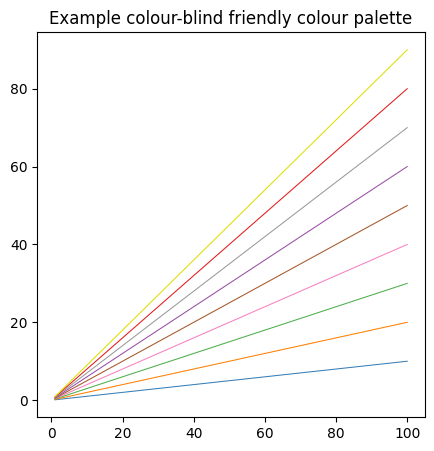
\includegraphics[width = 0.35\linewidth]{images/test_output_colourblind.png}
        \end{tabular}
        &\begin{tabular}{l}
            \parbox{0.5\linewidth}{%change the parbox width as appropiate
            We tried using a colour palette that is at least better than the standard colours used. Since we did not make many plots for our analysis (because there is not much use), this example plot shows the chosen colours.
            
            Furthermore, for plots we could have used shapes and forms to discern between different data sets or results.
            }
        \end{tabular} \\
    \end{tabular}
\end{frame}

%**************************************************************************
%\section{Bibliography} %**************************************************
%**************************************************************************
\setbeamertemplate{page number in head/foot}{}
\begin{frame}[noframenumbering]{References}
    %delete 'allowframebreaks' in the square bracket if there is only one frame with references to get rid of the numbering (i.e., References I, References II, ...)
    \printbibliography
\end{frame}

\begin{comment}
    \begin{tabular}{@{}ll@{}}  
        \begin{tabular}{l}
            \includegraphics[width = 0.35\linewidth]{images/}
        \end{tabular}
        &\begin{tabular}{l}
            \parbox{0.5\linewidth}{%change the parbox width as appropiate
            text
            }
        \end{tabular} \\
    \end{tabular}
\end{comment}